% Abstract file structure example : 
% \abstitle{title here}
% \absauthors{names and superscripts for affiliations here}
% \absaddress{affiliations, starting each one with its superscripts, separate affiliations with a \break}
% \abstext{
% \index{author abbreviated name, to be placed in authors' index}
% \index{create an index entry for each author}
%  The abstract text
% }

%% Abstract title
%\abstitle{Studio sui chirotteri troglofili della Grotta di Calafarina (Pachino, SR, Sicilia sud-orientale)}

%% Author names
%\absauthors{M. \textsc{Mucedda}$^1$,  G. \textsc{Fichera}$^2$, E. \textsc{Pidinchedda}$^1$}

%\absaddress{$^1$Centro Pipistrelli Sardegna, Via G. Leopardi 1 – 07100 Sassari, Italy - batsar@tiscali.it\break
%$^2$Universität Trier Universitätsring,15 - D-54286  Trier, Germany}

%% Abstract text
%\abstext{
%%% Author names for index. State each author separately using \index{Doe J.}
%\index{Mucedda M.}
%\index{Fichera G.}
%\index{Pidinchedda E.}
%%% The actual abstract text goes here
%} %% remember to close the abstract text block brace!!

\loadabstr[E018]{MUCEDDA M., FICHERA G., PIDINCHEDDA E. -- Studio sui chirotteri troglofili della Grotta di Calafarina (Pachino, SR, Sicilia sud-orientale)}{abstracts/extended_abstracts/C018_mucedda.ea_extended_title.tex}

\begin{multicols}{2}

\section*{Introduzione}
La Grotta di Calafarina, accatastata come SR 7011, è una cavità naturale situata nel comune di Pachino, che ospita nel suo interno una grande colonia di pipistrelli, che la rendono una delle più importanti della Sicilia.

Nel corso del biennio 2004--2005 è stato effettuato uno studio, con controlli periodici della popolazione di chirotteri all’interno della grotta, che è stato ripetuto nel triennio 2011-2013, allo scopo di stabilire quali specie siano presenti, accertarne l’entità numerica e ricostruire il loro ciclo biologico annuale. Brevi note sull’attività svolta nella prima fase compaiono in Mucedda \& Bertelli (2009).


\section*{Materiali e metodi}
Le visite di controllo all’interno della grotta sono state effettuate utilizzando materiali e attrezzature speleologiche. Per la documentazione fotografica sono state utilizzate macchine fotografiche digitali reflex Canon EOS 300D e 600D, con flash elettronici Canon Speedlite 550 EX e Metz 44. Il conteggio fotografico dei pipistrelli è stato realizzato al computer con un programma di grafica in modo preciso o comunque con un margine di errore estremamente ridotto.

Le catture dei pipistrelli ove necessario sono state realizzate con l’uso di retino e canna telescopica da 9 metri.

Le misurazioni biometriche degli animali sono state effettuate con un calibro della precisione di 0.1 mm e una pesola della precisione di 0.5 g.

Tutti gli esemplari sono stati prontamente liberati al termine delle operazioni. 

Le registrazioni dei suoni dei pipistrelli sono state effettuate con due Bat-detector Pettersson D980 e D240x, in modalità \textit{Time expansion}, più un registratore Zoom H2. Le elaborazioni al computer sono state realizzate con il programma Batsound della Pettersson.

Le temperature sono state misurate con un termometro digitale della precisione di 0.1\degree{}~C.

Per l'identificazione di \emph{Rhinolophus mehelyi} sono stati utilizzati i caratteri morfologici di Mucedda et al. (2009), mentre per \emph{Myotis myotis}/\emph{blythii} è stata usata la formula discriminante di Arlettaz (1995).

Tutte le fasi dello studio sono state realizzate seguendo le norme delle ``Linee guida per il monitoraggio dei Chirotteri'' (Agnelli et Al., 2004). 

Le attività sono state condotte con le autorizzazioni dell’Assessorato Regionale Territorio e Ambiente della Regione Sicilia (1814 del 26/05/2004 e 1742 del 01/06/2012) e del Ministero dell’Ambiente e della tutela del Territorio e del Mare (DPN/2D/2004/7489 del 15/03/2004 e 0009358 del 07/06/2012).

\subsection*{La grotta}
La Grotta di Calafarina è una cavità di origine carsica, situata lungo la zona costiera a sud di Marzamemi, nella estrema punta meridionale della Sicilia, che si apre con una piccola dolina di crollo a 15 m di quota, su una formazione calcarea miocenica di Calciruditi dell'Aquitaniano (Colacicchi, 1963). 

\begin{Figure} %[!ht]
  \centering\small
  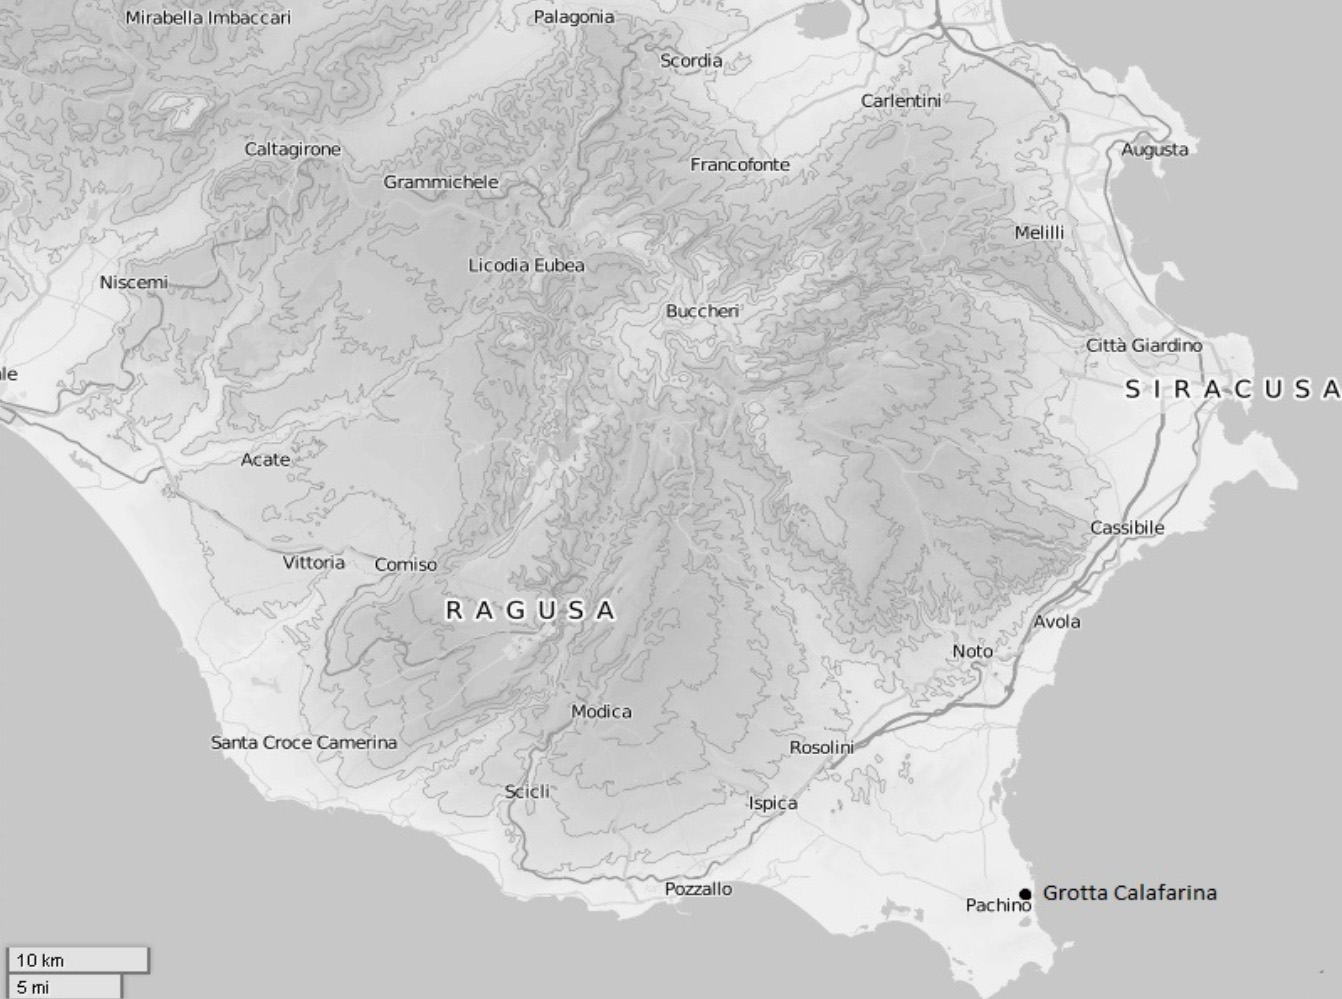
\includegraphics[width=\linewidth]{abstracts/extended_abstracts/C018_Figure1.png}
  \captionof*{}{Fig. 1 – Posizione geografica della Grotta di Calafarina.}
\end{Figure}
\begin{figure*}[t] %[!ht]
  \centering\small
  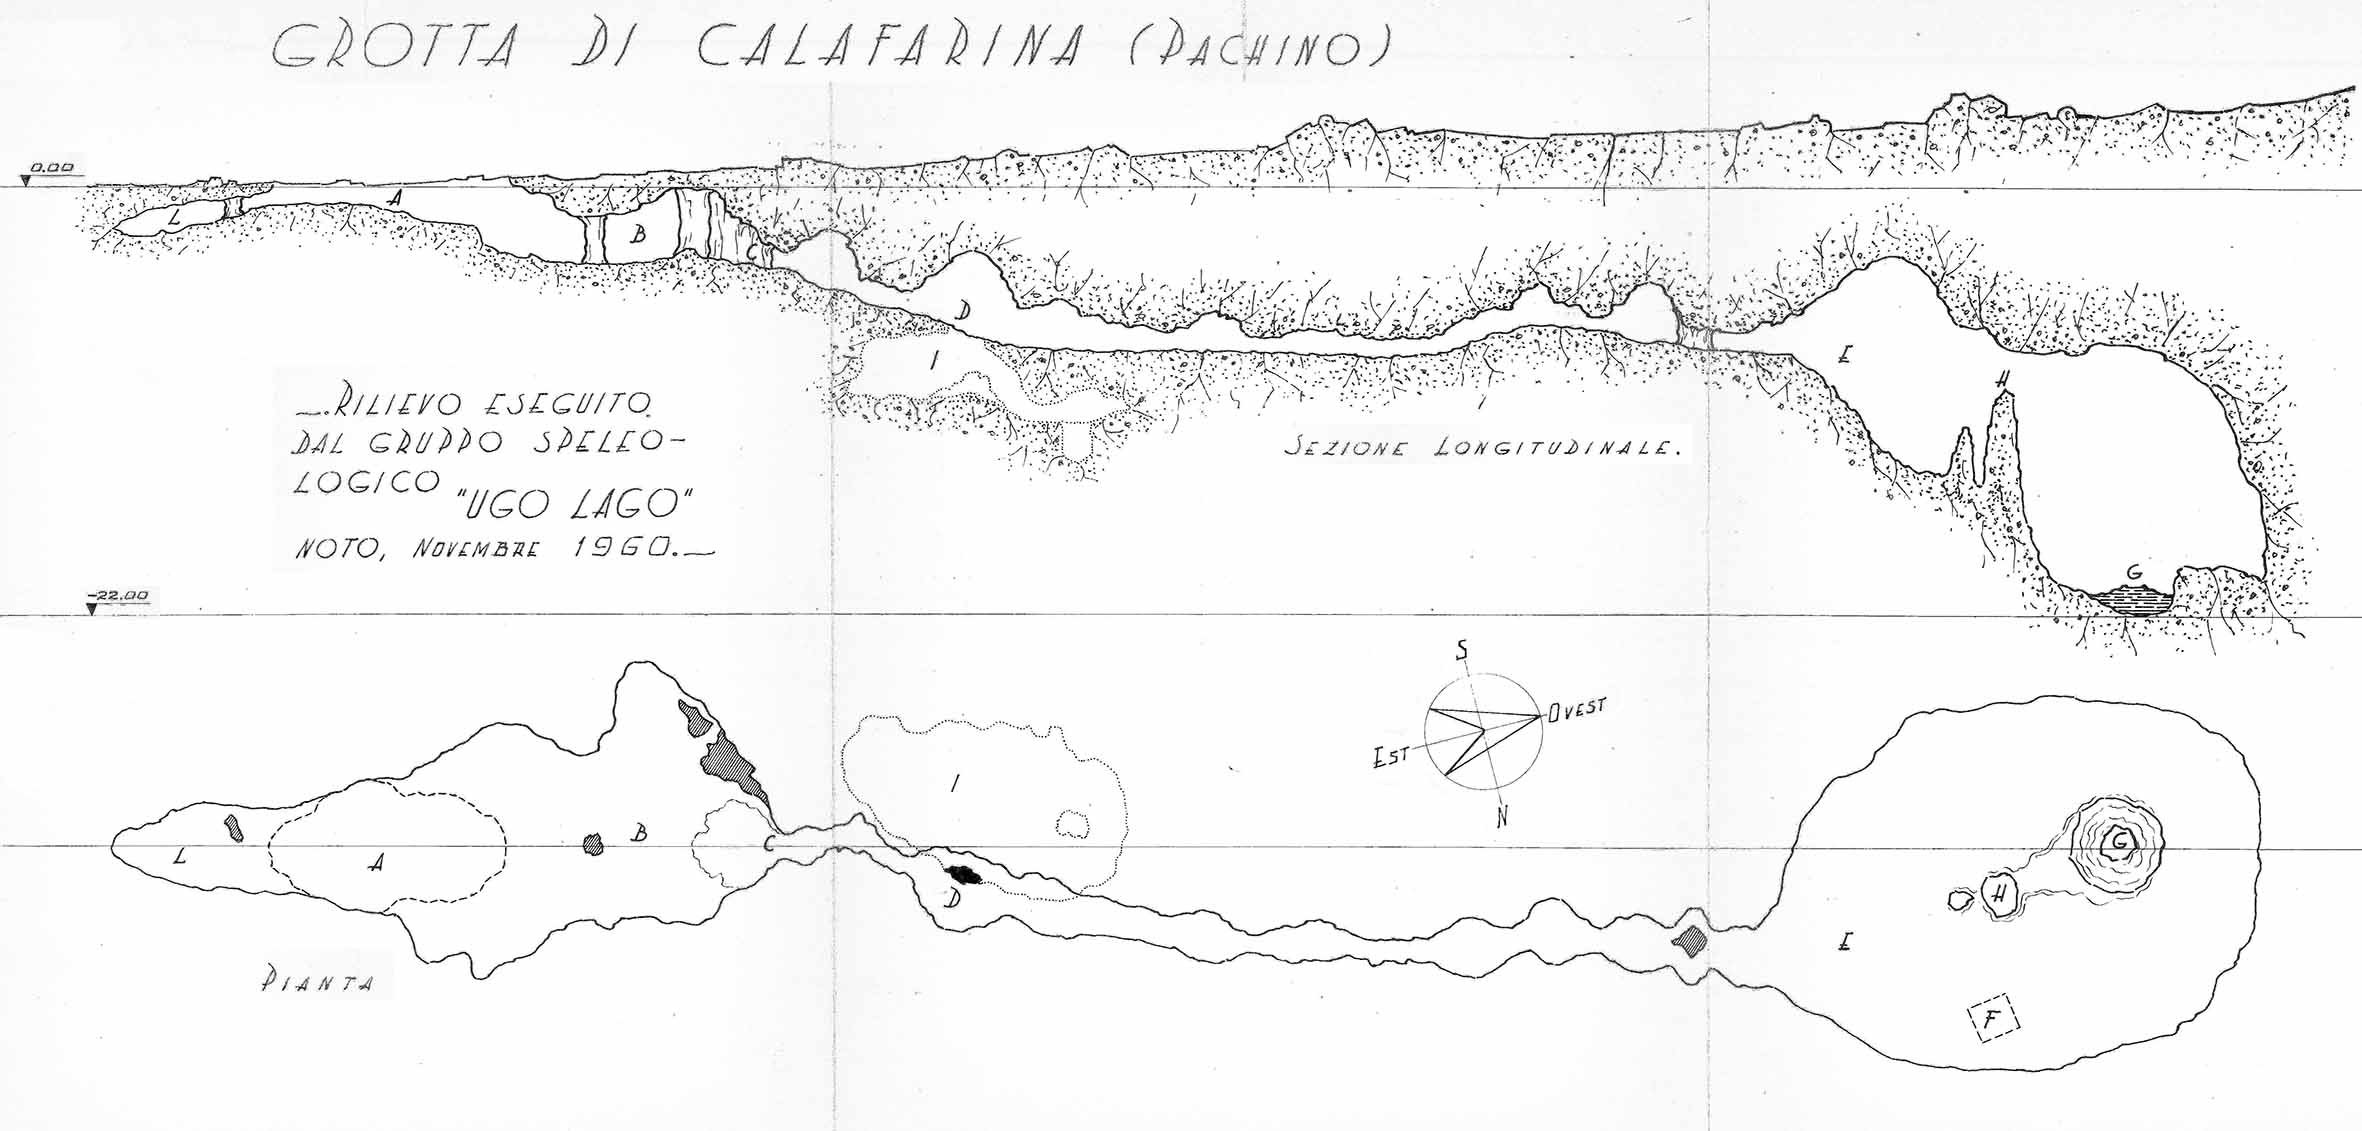
\includegraphics[width=\linewidth]{abstracts/extended_abstracts/C018_Figure2.png}
  \caption*{Fig. 2 – Rilievo topografico della grotta (Gruppo Speleologico ``Ugo Lago'').}
\end{figure*}

La cavità dopo l’ingresso presenta una salto verticale di circa 3 m e poi si sviluppa ad andamento sub orizzontale, con un disagevole cunicolo di circa 40 m che sbuca in un’ampia sala terminale discendente (la ``Camera dei Pipistrelli'' di Ragonese), di circa 20$\times$30 m, dove si stabilisce una grande colonia di pipistrelli. Sul lato destro della sala si innalza verso l’alto uno stretto pozzo artificiale di 10 m che proviene dalla superficie, che risulta essere attualmente occluso, ma che negli anni '60 risultava aperto e in parte rischiarava la sala (Ragonese, 1968). La grotta ha uno sviluppo orizzontale di 123 m e un dislivello di -22 m. La sua posizione è data dalle seguenti coordinate: Lat.  \ang{36;43;18.45}~N – Long. \ang{15;07;02.14}~E (WGS84 da GoogleEarth).

\begin{figure*}[t] %[!ht]
  \centering\small
  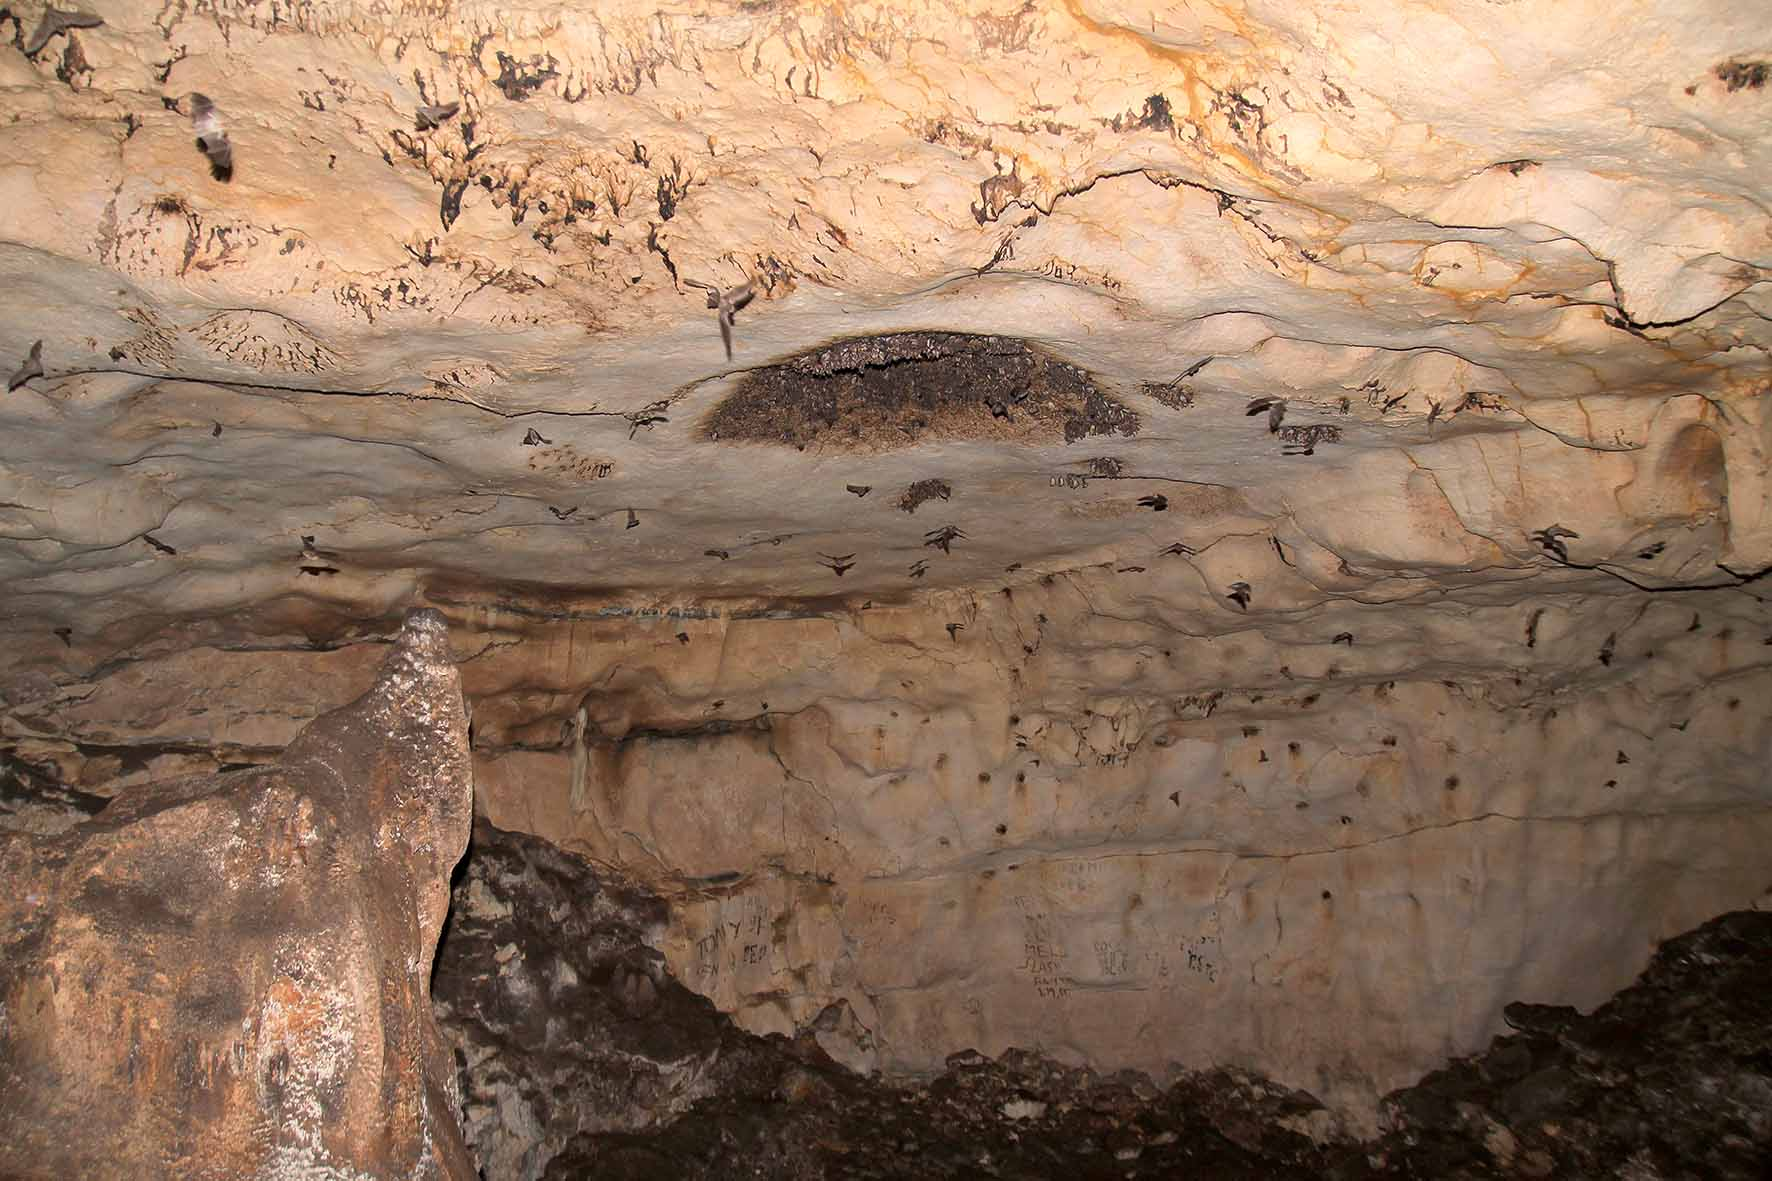
\includegraphics[width=\linewidth]{abstracts/extended_abstracts/C018_Figure3.png}
  \caption*{Fig. 3 - Veduta della sala terminale (Foto Gaetano Fichera).}
\end{figure*}

\subsection*{Note bibliografiche}
Il primo a darci notizia della presenza di pipistrelli nella Grotta di Calafarina è Orsi (1907), che descrive la cavità come ricchissima di guano e riferisce che l’ingresso della cavità, prima molto angusto, era stato allargato con l'utilizzo di mine.

La popolazione chirotterologica viene studiata per la prima volta da Ragonese (1967), del Gruppo Speleologico ``Ugo Lago'  di Noto, che la sceglie dal 1961 come stazione di inanellamento per i pipistrelli. Ragonese riferisce che la colonia è costituita da \emph{Rhinolophus ferrumequinum}, \emph{Myotis myotis} e \emph{Myotis capaccinii}, che arrivano a migliaia in aprile e maggio, le femmine partoriscono in estate e ripartono a settembre, asserendo che è un mistero dove essi vadano, mentre d'inverno c'è solo una decina di esemplari in semiletargo. Nel 1968 Ragonese pubblica un intero libro dal titolo ``Nel buio della Calafarina'' dedicato alla cavità in tutti i suoi aspetti descrittivi, archeologici e faunistici, confermando quanto già detto prima sui pipistrelli. Dice di aver inanellato 518 individui dal 9/7/1961 al 9/7/1967, la maggior parte dei quali sono \emph{M. myotis} (452), con pochi \emph{M. capaccinii} (61) e qualche  \emph{R. ferrumequinum} (5), riportando i dati in una lunga tabella.

\begin{figure*}[t] %[!ht]
  \centering\small
  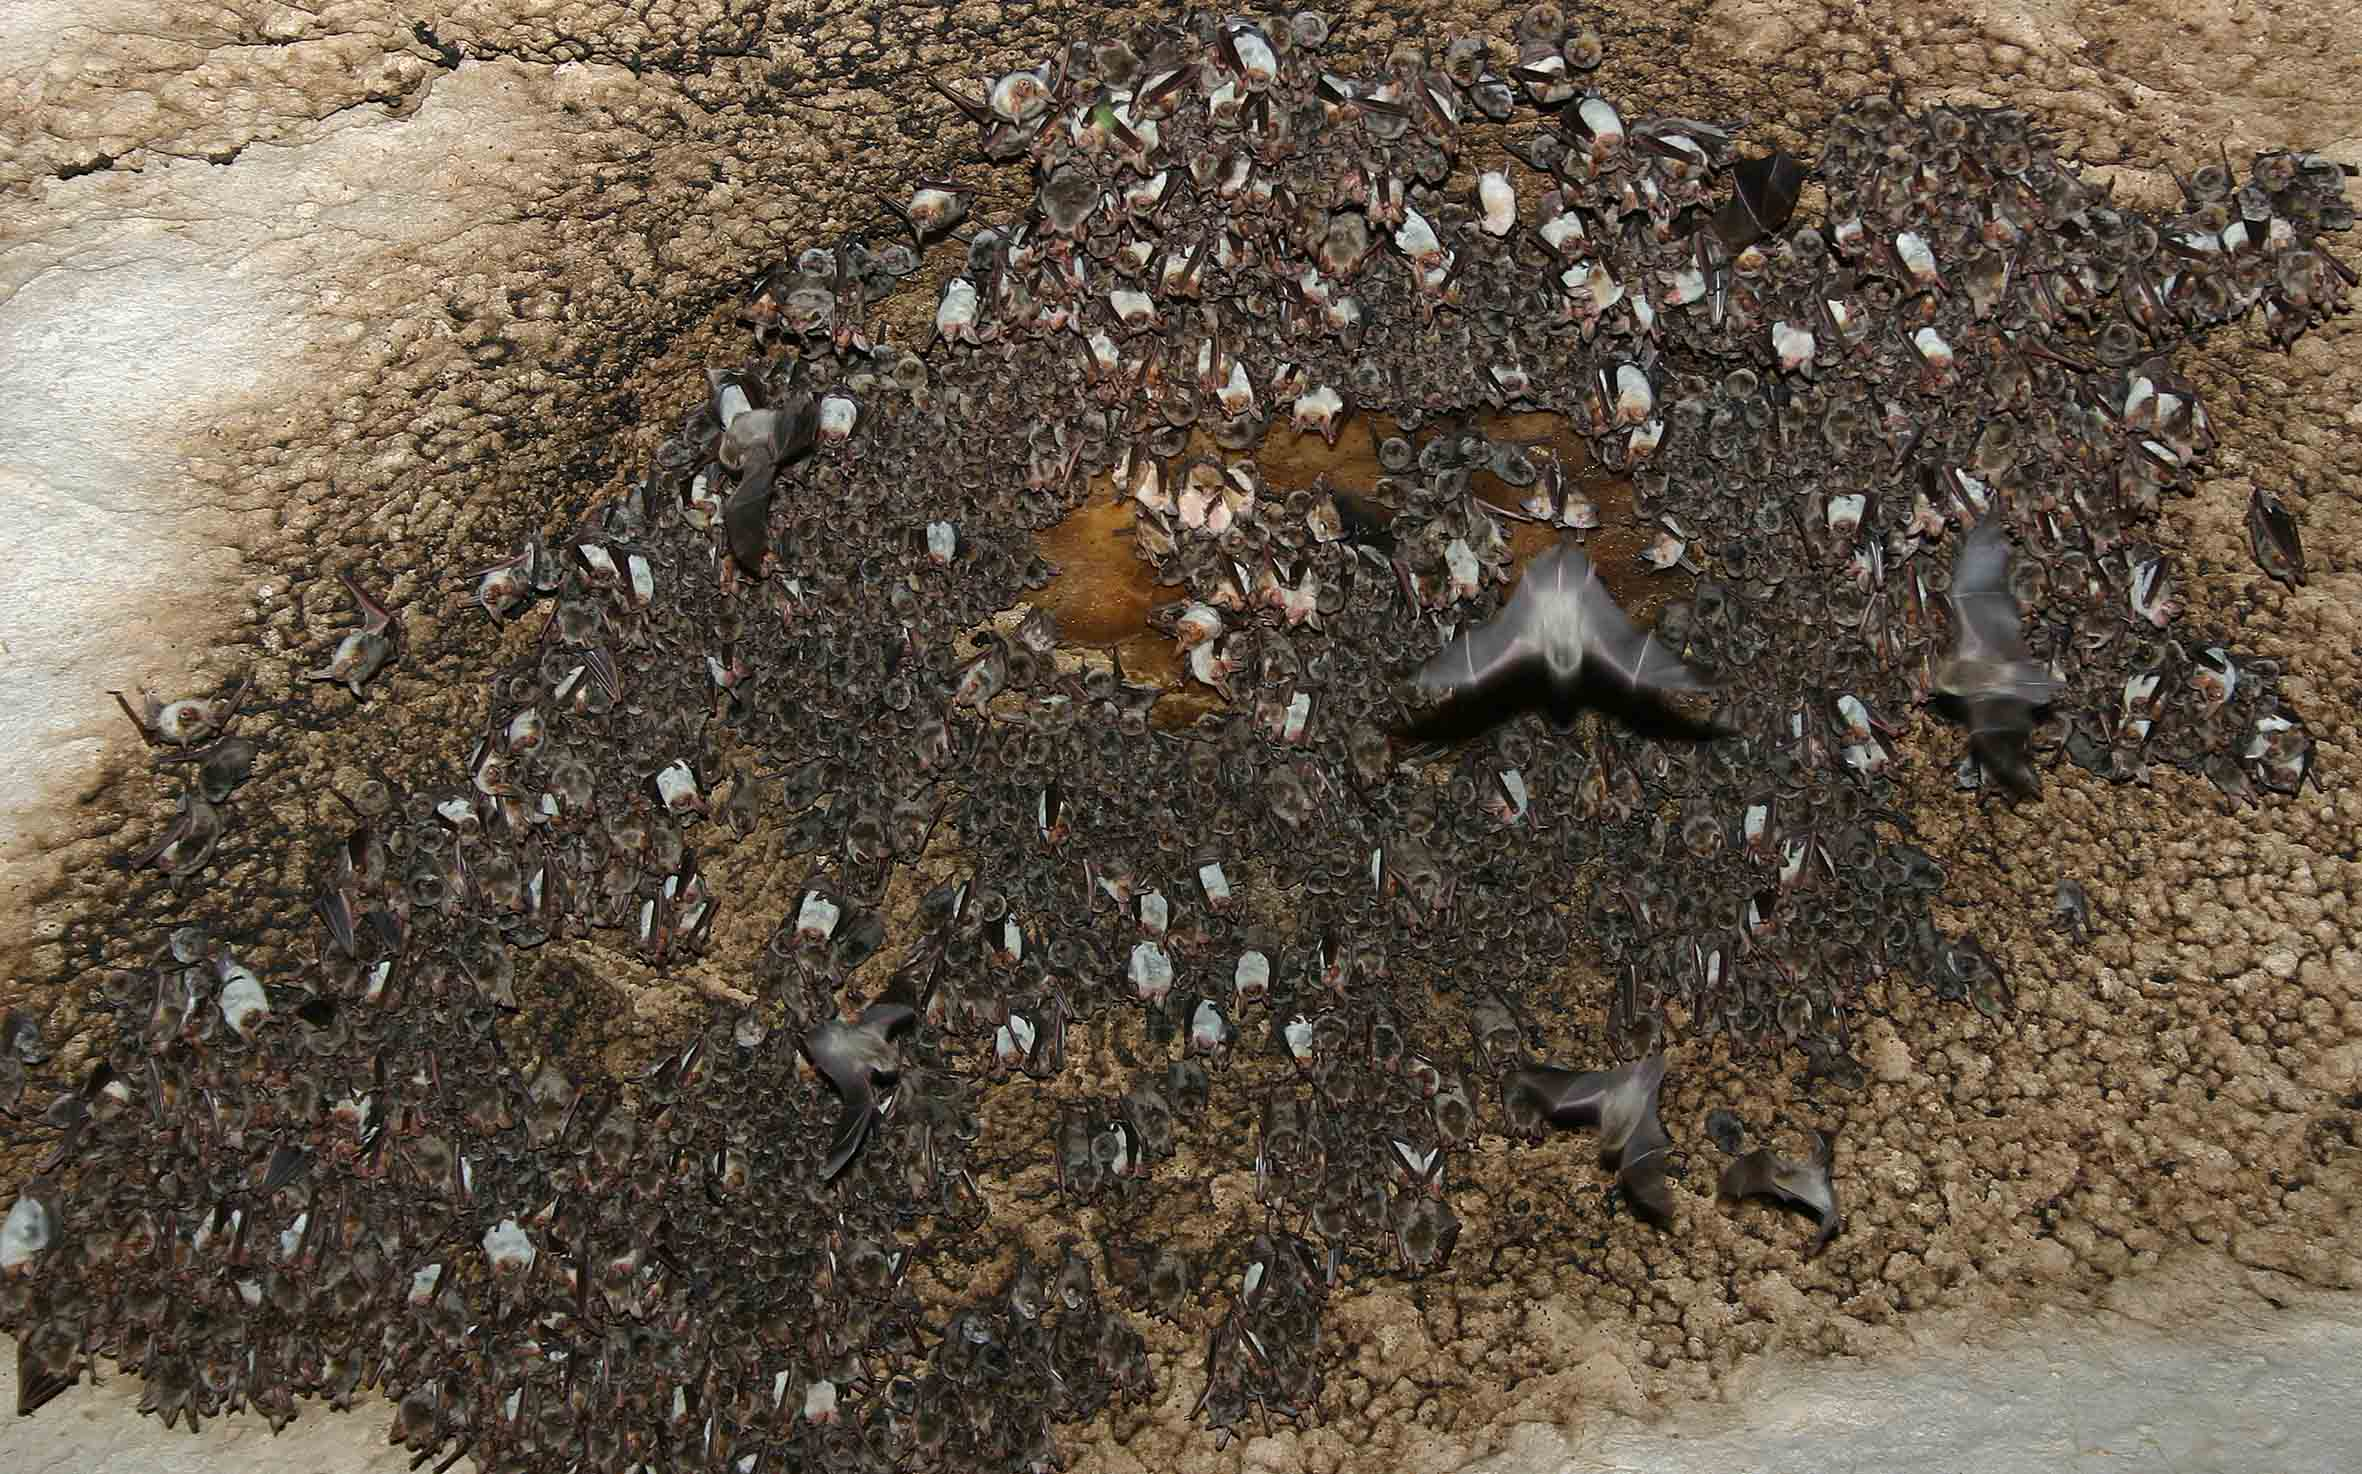
\includegraphics[width=\linewidth]{abstracts/extended_abstracts/C018_Figure4.png}
  \caption*{Fig. 4 – La colonia di pipistrelli nel mese di agosto (Foto Mauro Mucedda).}
\end{figure*}

Ragonese, con i suoi collaboratori, è stato probabilmente l’unico a studiare di persona i pipistrelli di Calafarina e pubblicare dati originali. I successivi autori infatti si limitano a citare i suoi lavori e i suoi dati, senza apparentemente aggiungere nulla di nuovo. Così Caruso (1978), Caruso e Costa (1978), Zava et Al. (1986), Caruso (1995), Caruso e Grasso (1996) per la grotta riportano tutti \emph{M. myotis}, \emph{M. capaccinii} e \emph{R. ferrumequinum}. Ragonese \& Contoli (1996) stranamente citano invece solo \emph{M. myotis} e \emph{M. capaccinii}.

Infine Mucedda et al. 2009 citano \emph{M. myotis}, \emph{M. capaccinii}, \emph{R. mehelyi} e \emph{M. schreibersii}, aggiungendo quindi le ultime due specie che sino ad allora non erano note per la cavità.

\section*{Risultati} 
Il nostro studio ha consentito di accertare nella grotta la presenza di 5 specie di chirotteri:
\begin{compactitem}
\item Rinolofo maggiore (\emph{Rhinolophus ferrumequinum} Schreber, 1774)
\item Rinolofo di Mehely (\emph{Rhinolophus mehelyi} Matschie, 1903)
\item Vespertilio maggiore (\emph{Myotis myotis} Borkhausen 1797)
\item Vespertilio di Capaccini (\emph{Myotis capaccinii} Bonaparte,1837)
\item Miniottero (\emph{Miniopterus schreibersii} Kuhl, 1817)
\end{compactitem}

I pipistrelli si radunano stagionalmente nell’ampia sala terminale, dove formano una grande colonia plurispecifica, che si aggrega principalmente in un nicchione del soffitto nella parte inferiore, e anche in gruppi minori in altre zone della sala. In altre parti della grotta sono stati osservati solo rari e occasionali esemplari. 

Numericamente la colonia risulta formata in massima parte da \emph{M. myotis} e da \emph{M. schreibersii}, che sono le specie preponderanti, e da un numero molto ridotto di \emph{M. capaccinii} e di \emph{R. mehelyi}. Il \emph{R. ferrumequinum} è stato osservato invece in pochi esemplari solamente in una occasione nel cunicolo che porta alla sala interna e quindi non si aggrega alle altre specie che formano la colonia.

La maggior parte dei pipistrelli non utilizza la grotta tutto l’anno, ma essi compiono dei movimenti migratori che li portano nella cavità generalmente in primavera, per poi gradualmente abbandonarla in autunno.

Qui di seguito riportiamo le osservazioni relative al ciclo annuale, con la dinamica della popolazione chirotterologica, nelle sue variazioni stagionali.

A causa della sua elevata temperatura interna, la Grotta di Calafarina non è idonea per il letargo, e pertanto in periodo invernale (dicembre-gennaio) sono presenti solo 30--40 esemplari tra \emph{M. schreibersii}, \emph{M. myotis} e \emph{M. capaccinii}. Già in febbraio si registra un lieve incremento nel numero di animali presenti nella Grotta, che possono arrivare a circa 200 esemplari.

In primavera la popolazione cresce notevolmente, con l’arrivo delle colonie migratorie dei pipistrelli, il cui numero in aprile raggiunge i 1300 esemplari e in maggio arriva a 1800, in gran parte \emph{M. myotis} e \emph{M. schreibersii}, con pochi \emph{M. capaccinii} e pochissimi \emph{R. mehelyi}; queste due ultime specie sono difficili da quantificare dato il loro esiguo numero rispetto alle due specie preponderanti. In questo periodo nel cunicolo di accesso alla sala terminale sono stati osservati anche alcuni \emph{R. ferrumequinum}, che costituiscono una presenza solo sporadica e occasionale nella grotta. Nel mese di maggio avvengono le prime nascite.

Nei mesi estivi la colonia cresce numericamente a seguito delle nascite, con oltre 2000 esemplari stimati, che rimane invariata in genere sino a settembre. E’ stata osservata la presenza di neonati di tutte e quattro le specie M. myotis, M. schreibersii, M. capaccinii e R. mehelyi.
Con l’arrivo dell’autunno si riscontra un calo numerico dei pipistrelli, che pian piano abbandonano la grotta diretti alle località di svernamento, riducendosi in novembre a qualche centinaio di esemplari. 

Nel corso del monitoraggio, a causa dei pipistrelli subito in movimento e le conseguenti difficoltà, il numero dei pipistrelli è stato spesso stimato. Solo in alcune occasioni nella colonia si sono potuti eseguire conteggi fotografici esatti degli animali, con i seguenti risultati:
\begin{compactitem}
\item 27 agosto 2004: 506 \emph{M. myotis}, 810 \emph{M. schreibersii}, 19 \emph{R. mehelyi} e 28 \emph{M. capaccinii}.
\item 27 aprile 2005: 570 \emph{M. myotis}, 820 \emph{M. schreibersii}, 4 \emph{R. mehelyi}.
\item 6 maggio 2013: 789 \emph{M. myotis}, 1082 \emph{M. schreibersii}, 6 \emph{R. mehelyi}.
\end{compactitem}

Come già detto, la Grotta di Calafarina è una cavità molto calda. Le temperature misurate nella Sala dei Pipistrelli infatti oscillano nel corso dell’anno tra 21\celsius{} e 22\celsius{}, che data l’elevata umidità degli ambienti sotterranei rendono la presenza dell’uomo all’interno particolarmente problematica. È incredibile come a queste temperature sia possibile riscontrare pipistrelli in letargo, anche se solo poche decine di esemplari.

Il Rinolofo di Mehely è stato oggetto anche di un’indagine bioacustica, basata sulla registrazione dei suoni di un limitato numero di esemplari, tenendo gli animali fermi in mano a una distanza di 30 cm dal microfono del Bat detector, come indicato in Russo et al. (2007). Gli individui di \emph{R. mehelyi} da noi analizzati in Sicilia mostrano una frequenza media dei segnali emessi più alta di quelli della Sardegna. Gli esemplari sardi infatti hanno registrato valori di 104.3--109.8 kHz di frequenza, mentre i pochi campioni esaminati di Calafarina hanno registrato valori di 111.4--113.2 kHz. L’argomento meriterebbe ulteriori indagini di approfondimento.

\section*{Discussione}
Il monitoraggio ha consentito di stabilire che la Grotta di Calafarina è un sito di riproduzione, con la presenza di una colonia \textit{nursery} composta da 4 specie di pipistrelli: \emph{Miniopterus schreibersii}, \emph{Myotis myotis}, \emph{Myotis capaccini} e \emph{Rhinolophus mehelyi}, con la preponderanza numerica delle prime due.

Questo tipo di aggregazione mista è molto frequente per i chirotteri troglofili in ambiente cavernicolo, riscontrata spesso in Sardegna (Mucedda et al., 1995), in Corsica (Courtois et al., 2011) e in Sicilia (Mucedda et al., in stampa), sia con tutte e quattro le specie insieme che con sole tre di esse.

Il \emph{Rhinolophus ferrumequinum} è invece occasionale e non si riproduce in questa cavità, in quanto, come è noto questa specie nel periodo estivo abbandona le grotte e preferisce utilizzare rifugi quali edifici, cavità artificiali più asciutte e altre tipologie di strutture.

La colonia riproduttiva della Grotta Calafarina è una delle più importanti della Sicilia e geograficamente risulta essere allo stato attuale la più meridionale d'Italia. In Sicilia orientale per entità numerica è seconda solo alla Grotta dei Pipistrelli di Pantalica, dove in estate si aggregano sino a 4000 chirotteri (Mucedda et al., in stampa).

Le nascite hanno inizio nella prima decade del mese di maggio con i primi parti di \emph{Myotis capaccinii} e \emph{Myotis myotis}. I \emph{Miniopterus schreibersii} partoriscono invece poco più tardi a fine maggio e in giugno. I \emph{Rhinolophus mehelyi} partoriscono per ultimi in giugno.

Terminato il periodo riproduttivo, ha inizio la fase degli accoppiamenti e in agosto e in settembre sono state osservate coppie di \emph{Myotis myotis}, isolate dalla colonia principale.

Non sono emerse variazioni di rilievo tra le osservazioni del 2004--2005 e quelle del 2011--2013, per cui si ritiene che a distanza di 7--8 anni la popolazione di chirotteri della Grotta di Calafarina sia al momento stabile e quindi non soffra di particolari pressioni.

Tra le specie di pipistrelli che utilizzano la grotta, possiamo considerare il \emph{Rhinolophus mehelyi} come quello più rilevante dal punto di vista protezionistico. La sua presenza è particolarmente importante perché in tutta la Sicilia sono note attualmente due sole stazioni per questa specie e quella di Calafarina risulta essere sino ad oggi l’unica colonia riproduttiva attualmente nota nella regione (Mucedda et al. 2009). 

Il Rinolofo di Mehely si aggrega con le altre specie nella colonia, ma è numericamente molto ridotto. Nel corso dei monitoraggi, nel periodo estivo sono stati osservati tra un minimo di 7 e un massimo di 20 esemplari. È presente anche in autunno, ma in periodo invernale risulta invece assente. Si tratta pertanto di una specie particolarmente minacciata, in posizione talmente critica da poterla definire ``quasi in via di estinzione'' per la Sicilia.

\subsection*{Confronti con il passato}
È interessante notare che la colonia di pipistrelli è passata indenne nel tempo a grandi rimaneggiamenti che hanno interessato la Grotta di Calafarina, quali l’allargamento dell’ingresso con le mine, lo scavo del pozzo artificiale nella sala terminale e i lavori di estrazione del guano. È questo proprio un caso di adattamento da parte dei chirotteri, che sino ai giorni nostri continuano ad utilizzare la cavità come rifugio, nonostante le azioni di pesante disturbo succedutesi nel tempo.

Osservando i dati storici, la tipologia dei movimenti migratori stagionali da noi riscontrati nella grotta appare analoga a quanto osservato negli anni ’60 da Ragonese (1967, 1968).

Differenze sostanziali risultano invece riguardo alle specie presenti. Ragonese infatti parla di una colonia formata da soli \emph{R. ferrumequinum}, \emph{M. myotis} e \emph{M. capaccinii}, mentre attualmente risultano presenti anche \emph{R. mehelyi} e \emph{M. schreibersii} che prima non erano stati riscontrati. Sulla base di queste considerazioni, si potrebbero ipotizzare due possibilità: Ragonese potrebbe aver commesso un errore nella identificazione e potrebbero essere sfuggite queste due ultime specie, oppure più probabilmente nell’arco di 50 anni la popolazione di chirotteri ha subito delle modificazioni sostanziali. Poichè lo stesso Ragonese (1968) dichiara che all’epoca il pozzo interno che sbuca in superficie era aperto, si potrebbe pensare che la chiusura di tale pozzo (che non si sa quando sia avvenuta) abbia modificato le caratteristiche climatiche della grotta (circolazione d’aria, umidità e temperatura), e si siano create condizioni più idonee alle due specie \emph{R. mehelyi} e \emph{M. schreibersii} che hanno così iniziato a frequentare la grotta. 

Appare comunque strano che \emph{R. ferrumequinum} risultasse presente in passato nella colonia estiva, perché come già detto questa specie in estate è solita trasferirsi in altri rifugi quali edifici e cavità artificiali.

Come già visto in precedenza, Ragonese aveva inanellato nell’arco di 6 anni 452 \emph{M. myotis}, 61 \emph{M. capaccinii} e 5 \emph{R. ferrumequinum}, per un totale di 518 individui. Andando ad esaminare i dati in modo più approfondito, risulta che i \emph{M. myotis} erano 225 femmine, 214 maschi e 13 indeterminati, i \emph{M. capaccinii} 49 femmine e 12 maschi e i \emph{R. ferrumequinum} 1 femmina, 3 maschi e 1 indeterminato. Benchè non sia possibile conoscere la situazione della totalità degli animali presenti, si evidenzia che la colonia di riproduzione non era costituita da sole femmine (54.6\% delle catture), ma il numero dei maschi presenti era sempre notevole (45.4\% delle catture). L’inanellamento di soli 5 \emph{R. ferrumequinum} sembrerebbe confermare che questa specie non fosse numerosa ma solo occasionale. Esaminando i dati pubblicati, risulta che nell’arco dei 6 anni di attività si sono registrate solo 3 ricatture. Questo fa pensare che la colonia possa aver risentito delle attività di inanellamento e molti pipistrelli nel tempo abbiano probabilmente preferito non ritornare nella grotta.

Poco si può ipotizzare sugli spostamenti migratori. Sino ad oggi non sono note in Sicilia colonie di letargo invernale di \emph{Myotis myotis}, se non rifugi di pochi esemplari, per cui rimangono sconosciute le località in cui si trasferisce questa specie. Per \emph{M. schreibersii} e \emph{M. capaccini} sono invece note delle colonie invernali sull’Etna (Fichera et al., in stampa), per cui è probabile ritenere che essi possano trascorrere il letargo proprio sull’Etna. 

L’identificazione dei \emph{M. myotis} è stata effettuata su un numero ridotto di esemplari, basandosi sulle misurazioni biometriche di avambraccio e orecchio col metodo di Arlettaz (1995). Nella gran moltitudine di pipistrelli della colonia non possiamo comunque escludere la presenza anche di esemplari di \emph{M. blythii}, che spesso forma colonie miste col \emph{M. myotis}, e questa problematica richiederebbe un approfondimento. Sinora comunque non risultano note in Sicilia colonie di riproduzione con entrambe le specie.

\subsection*{L’estrazione del guano}
Orsi (1907) riferisce che la Grotta di Calafarina era ricchissima di guano, che veniva estratto dal proprietario, il Marchese Antonio Di Rudinì, utilizzandolo per fertilizzare le proprie terre. Ragonese (1968) ritiene che il pozzo artificiale che si innalza nella sala terminale era stato forse scavato dal Marchese, proprio per l’estrazione del guano. La presenza di grandi depositi di guano è la testimonianza della frequentazione da parte dei chirotteri da tempi molto lontani. Non si hanno però informazioni dettagliate sulle quantità estratte e sul periodo esatto in cui abbia avuto luogo l’attività estrattiva. 

Un’altro riferimento bibliografico su questo tema è quello di Paris (1899), che cita analisi di guano proveniente da Pachino, riferibile molto probabilmente alla Grotta di Calafarina. 

\subsection*{Interventi di tutela}
Data l’importanza della popolazione di pipistrelli della Grotta di Calafarina, le cui specie sono tutte inserite in Allegato II della Direttiva Habitat, sarebbero auspicabili degli interventi di tutela, almeno per evitare che persone incontrollate accedano alla sala terminale, arrecando grave disturbo alla colonia. 

Il sito è infatti privo di protezioni e pertanto potenzialmente minacciato, data la sua facilità di accesso e notorietà presso la popolazione locale. Sarebbe necessario sensibilizzare gli abitanti del luogo, con attività divulgative e cartellonistica appropriata.

Si deve segnalare che qualora, per malaugurata ipotesi, qualcuno dovesse riaprire l’imbocco del pozzo esterno posto nella sala terminale, si avrebbero delle gravi modificazioni nelle caratteristiche ambientali della grotta, con rischio elevato di perdita della colonia di pipistrelli.

Non è facile prevedere un intervento di tutela della grotta, perché la cavità è molto conosciuta e frequentata dalla gente del posto, soprattutto i ragazzi di Pachino e Portopalo.

Per un intervento attivo di tutela, occorre tenere presente che non è possibile l’installazione di un cancello a totale chiusura dell’ingresso della grotta, perché i Miniotteri non sono in grado di passare attraverso le sbarre, come è già successo nella Grotta Palombara di Melilli (Mucedda et al., in stampa). Anziché un cancello si potrebbe prevedere una recinzione alta intorno all’imbocco, ma si deve segnalare che una recinzione installata in passato era già stata abbattuta.

\vskip3mm

\begin{small}
\noindent\textbf{Ringraziamenti}\\
Si ringraziano il Centro Speleologico Etneo, Rosario Ardilio, Maria Luisa Bertelli, Mariacristina Borrello, Federica Calabrese, Dalma Cultrera, Sergio Firinu, Iolanda Galletti, Tiziana Grech, Domenico Longo, Fabio Morreale, Michele Nanzarelli, Alfio Nicolosi, Giorgio Sabella che hanno partecipato alle attività o ci hanno fornito utili informazioni per le indagini.

\vskip3mm

\noindent\textbf{Bibliografia}\\

Agnelli P., Martinoli A., Patriarca E., Russo D., Scaravelli D., Genovesi P. (Eds.), 2004. Linee guida per il monitoraggio dei Chirotteri: indicazioni metodologiche per lo studio e la conservazione dei pipistrelli in Italia. Quad. Cons. Natura 19, Min. Ambiente-Ist. Naz. Fauna Selvatica.

Arlettaz R., 1995. \emph{Myotis myotis} – \emph{Myotis blythii}. Ecology of the sibling mouse-eared bats, Horus Publishers Martigny, Switzerland, 44--52.

Caruso D., 1978. Il popolamento cavernicolo della Sicilia (Ricerche faunistiche ed ecologiche sulle grotte di Sicilia. VII). Lav. Soc. Ital. Biogeogr. Nuova serie, Vol. VII (Pubblicato 1982): 587--614. 

Caruso D., 1995. L’attuale stato delle conoscenze sulla fauna delle grotte di Sicilia (Ricerche faunistiche ed ecologiche sulla grotte di Sicilia. VIII). Atti I Convegno Regionale di Speleologia della Sicilia, Ragusa 1990, Vol. II: 349--378.

Caruso D., Costa G., 1978. Ricerche faunistiche ed ecologiche sulle grotte di Sicilia. VI – Fauna cavernicola di Sicilia (Catalogo ragionato). Animalia, Catania, 5 (1--3): 423-513.

Caruso D., Grasso R., 1996. La fauna delle grotte. Atti Convegno ` La fauna degli Iblei' , Noto, 1995: 201--281.

Colacicchi R., 1963. Geologia del territorio di Pachino (Sicilia meridionale). Geologia romana, II, 1963, pp. 343--404.

Courtois J.Y., Rist D., Beuneux G., 2011. Les chauves-souris de Corse. Albiana, Ajaccio: pp. 167.

Fichera G., Mucedda M., Pidinchedda E., Catalano P. Sperlinga G., (in stampa). Aggiornamento delle conoscenze sulla chirotterofauna del comprensorio etneo (Sicilia orientale). In: Madonia G., Panzica La Manna M., Vattano M. (Eds.) Atti del 5\degree{} Congresso Regionale di Speleologia della Sicilia, 23--24 novembre 2013, Castello di Rampinzeri, Santa Ninfa (TP).

Mucedda M., Castorina R., Fichera G., Pidinchedda E., (in stampa). Osservazioni sui pipistrelli di due importanti grotte degli Iblei: la Grotta Palombara (Melilli) e la Grotta di Pantalica (Sortino) (Sicilia orientale). In: Madonia G., Panzica La Manna M., Vattano M. (Eds.) Atti del 5\degree{} Congresso Regionale di Speleologia della Sicilia, 23--24 novembre 2013, Castello di Rampinzeri, Santa Ninfa (TP).

Mucedda M., Pidinchedda, Bertelli M. L., 2009. Status del Rinolofo di Mehely (\emph{Rhinolophus mehelyi}) (Chiroptera, Rhinolophidae) in Italia. Atti del 2\degree{} Convegno Italiano sui Chirotteri, Serra San Quirico (AN), 21--23 novembre 2008: 89--98.

Mucedda M., Bertelli M.L., 2009. Cronache sulle ricerche di pipistrelli in Sicilia nel 2004 e 2005. Bollettino del Gruppo Speleologico  Sassarese, n. 19, 19--27.

Mucedda M., Murittu G., Oppes A., Pidinchedda E., 1995. Osservazioni sui Chirotteri troglofili della Sardegna. Boll. Soc. Sarda Sci. Nat., 30: 97--129.

Orsi P., 1907. La grotta di Calafarina presso Pachino (Siracusa), abitazione e sepolcro. Bullettino di Paletnologia Italiana, XXXIII: 7--22.
 
Paris G., 1899. Su di un nuovo guano di pipistrello trovato a Cagliari. Le Staz. Sperim. Agr. Ital., Modena 32, pp. 176--185.

Ragonese B., 1967. L'inanellamento dei pipistrelli in Sicilia,  Selecta n 10, Anno scolastco 1965--1966, Grafiche S. Corrado, Noto: 2--6.

Ragonese B., 1968. Nel buio di Calafarina. Ed. Ciranna, Roma, 133 pp.

Ragonese B., Contoli L., 1996. La mammalofauna. Atti Convegno ``La fauna degli Iblei'', Noto 1995: 123--129.

Russo D., Mucedda M., Bello M., Biscardi S., Pidinchedda E., Jones G., 2007. Divergent echolocation call frequencies in insular rhinolophids (Chiroptera): a case of character displacement? Journal of Biogeography 34: 2129-2138.

Zava B., Corrao, A.,  Catalano E., 1986. Chirotteri cavernicoli di Sicilia. Atti del IX Congreso Internacional de Espeleologia, Barcellona, Vol. II: 187--189.
\end{small}

\end{multicols}
% % EOF % %